\documentclass[11pt,a4paper]{report}
\usepackage[textwidth=37em,vmargin=30mm]{geometry}
\usepackage{calc,xunicode,amsmath,amssymb,paralist,enumitem,tabu,booktabs,datetime2,xeCJK,xeCJKfntef,listings}
\usepackage{tocloft,fancyhdr,tcolorbox,xcolor,graphicx,eso-pic,xltxtra,xelatexemoji}

\newcommand{\envyear}[0]{2025}
\newcommand{\envdatestr}[0]{2025-07-10}
\newcommand{\envfinaldir}[0]{webdb/2025/20250710/final}

\usepackage[hidelinks]{hyperref}
\hypersetup{
    colorlinks=false,
    pdfpagemode=FullScreen,
    pdftitle={Web Digest - \envdatestr}
}

\setlength{\cftbeforechapskip}{10pt}
\renewcommand{\cftchapfont}{\rmfamily\bfseries\large\raggedright}
\setlength{\cftbeforesecskip}{2pt}
\renewcommand{\cftsecfont}{\sffamily\small\raggedright}

\setdefaultleftmargin{2em}{2em}{1em}{1em}{1em}{1em}

\usepackage{xeCJK,xeCJKfntef}
\xeCJKsetup{PunctStyle=plain,RubberPunctSkip=false,CJKglue=\strut\hskip 0pt plus 0.1em minus 0.05em,CJKecglue=\strut\hskip 0.22em plus 0.2em}
\XeTeXlinebreaklocale "zh"
\XeTeXlinebreakskip = 0pt


\setmainfont{Brygada 1918}
\setromanfont{Brygada 1918}
\setsansfont{IBM Plex Sans}
\setmonofont{JetBrains Mono NL}
\setCJKmainfont{Noto Serif CJK SC}
\setCJKromanfont{Noto Serif CJK SC}
\setCJKsansfont{Noto Sans CJK SC}
\setCJKmonofont{Noto Sans CJK SC}

\setlength{\parindent}{0pt}
\setlength{\parskip}{8pt}
\linespread{1.15}

\lstset{
	basicstyle=\ttfamily\footnotesize,
	numbersep=5pt,
	backgroundcolor=\color{black!5},
	showspaces=false,
	showstringspaces=false,
	showtabs=false,
	tabsize=2,
	captionpos=b,
	breaklines=true,
	breakatwhitespace=true,
	breakautoindent=true,
	linewidth=\textwidth
}






\newcommand{\coverpic}[2]{
    % argv: itemurl, authorname
    Cover photo by #2~~(\href{#1}{#1})
}
\newcommand{\makeheader}[0]{
    \begin{titlepage}
        % \newgeometry{hmargin=15mm,tmargin=21mm,bmargin=12mm}
        \begin{center}
            
            \rmfamily\scshape
            \fontspec{BaskervilleF}
            \fontspec{Old Standard}
            \fontsize{59pt}{70pt}\selectfont
            WEB\hfill DIGEST
            
            \vfill
            % \vskip 30pt
            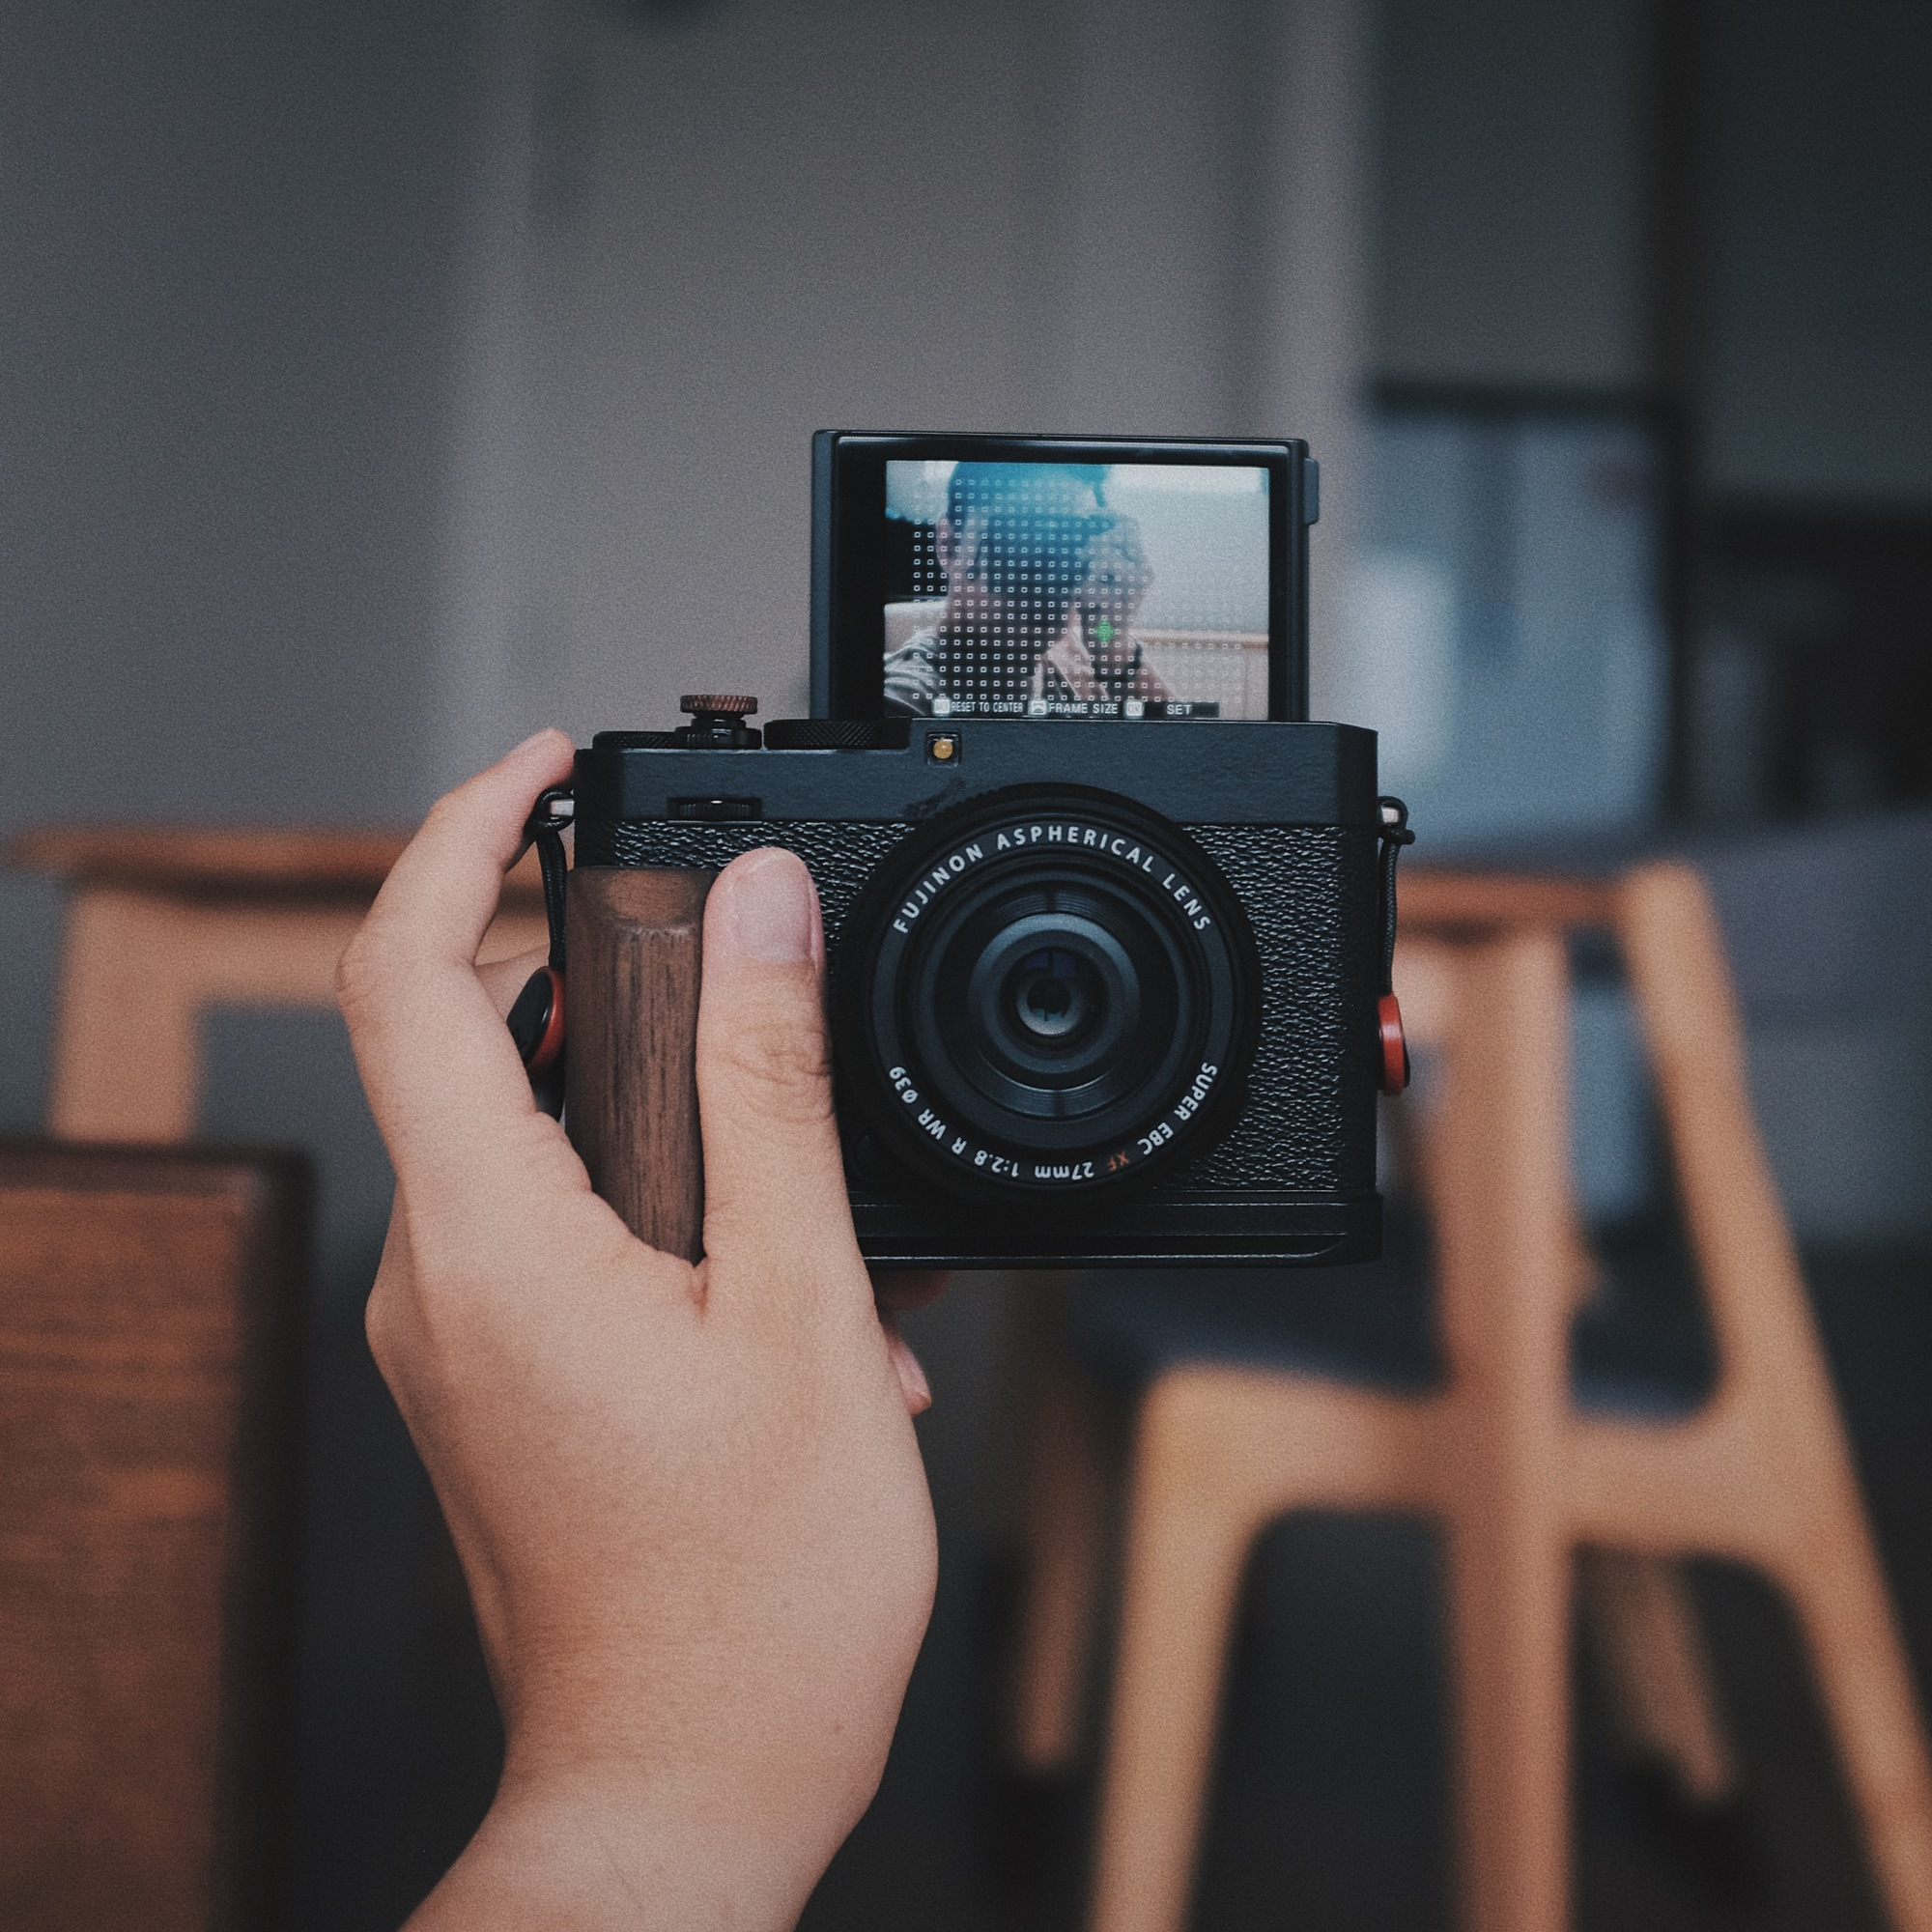
\includegraphics[width=\linewidth]{\envfinaldir/coverpic-prod.jpg}\par
            % \vskip 30pt
            \vfill

            \normalsize\rmfamily\scshape
            \copyright{} The Web Digest Project \hfill\large \envdatestr
        \end{center}
    \end{titlepage}
    % \restoregeometry
}
\newcommand{\simplehref}[1]{%
    \textcolor{blue!80!green}{\href{#1}{#1}}%
}
\renewcommand{\contentsname}{\center\Huge\sffamily\bfseries Contents\par\vskip 20pt}
\newcounter{ipartcounter}
\setcounter{ipartcounter}{0}
\newcommand{\ipart}[1]{
    % \vskip 20pt
    \clearpage
    \stepcounter{ipartcounter}
    \phantomsection
    \addcontentsline{toc}{chapter}{#1}
    % \begin{center}
    %     \Huge
    %     \sffamily\bfseries
    %     #1
    % \end{center}
    % \vskip 20pt plus 7pt
}
\newcounter{ichaptercounter}
\setcounter{ichaptercounter}{0}
\newcommand{\ichapter}[1]{
    % \vskip 20pt
    \clearpage
    \stepcounter{ichaptercounter}
    \phantomsection
    \addcontentsline{toc}{section}{\numberline{\arabic{ichaptercounter}}#1}
    \begin{center}
        \Huge
        \sffamily\bfseries
        #1
    \end{center}
    \vskip 20pt plus 7pt
}
\newcommand{\entrytitlefont}[1]{\subsection*{\raggedright\Large\sffamily\bfseries#1}}
\newcommand{\entryitemGeneric}[2]{
    % argv: title, url
    \parbox{\linewidth}{
        \entrytitlefont{#1}\par\vskip 5pt
        \footnotesize\ttfamily\mdseries
        \simplehref{#2}
    }\vskip 11pt plus 11pt minus 1pt
}
\newcommand{\entryitemGithub}[3]{
    % argv: title, url, desc
    \parbox{\linewidth}{
        \entrytitlefont{#1}\par\vskip 5pt
        \footnotesize\ttfamily\mdseries
        \simplehref{#2}\par\vskip 5pt
        \small\rmfamily\mdseries#3
    }\vskip 11pt plus 11pt minus 1pt
}
\newcommand{\entryitemAp}[3]{
    % argv: title, url, desc
    \parbox{\linewidth}{
        \entrytitlefont{#1}\par\vskip 5pt
        \footnotesize\ttfamily\mdseries
        \simplehref{#2}\par\vskip 5pt
        \small\rmfamily\mdseries#3
    }\vskip 11pt plus 11pt minus 1pt
}
\newcommand{\entryitemHackernews}[3]{
    % argv: title, hnurl, rawurl
    % \parbox{\linewidth}{
    %     \entrytitlefont{#1}\par\vskip 5pt
    %     \footnotesize\ttfamily\mdseries
    %     \simplehref{#3}\par
    %     \textcolor{black!50}{\href{#2}{#2}}
    % }\vskip 11pt plus 11pt minus 1pt
    \begin{minipage}{\linewidth}
            \entrytitlefont{#1}\par\vskip 5pt
            \footnotesize\ttfamily\mdseries
            \simplehref{#3}\par
            \textcolor{black!50}{\href{#2}{#2}}
    \end{minipage}\par\vskip 11pt plus 11pt minus 1pt
}







\begin{document}

\makeheader

\tableofcontents\clearpage




\ipart{Developers}
\ichapter{Hacker News}
\entryitemTwoLinks{Biomni: A General-Purpose Biomedical AI Agent}{https://news.ycombinator.com/item?id=44513843}{https://github.com/snap-stanford/Biomni}

\entryitemTwoLinks{Let Kids Be Loud}{https://news.ycombinator.com/item?id=44513801}{https://www.afterbabel.com/p/let-kids-be-loud}

\entryitemTwoLinks{Show HN: FlopperZiro – A DIY open-source Flipper Zero clone}{https://news.ycombinator.com/item?id=44512763}{https://github.com/lraton/FlopperZiro}

\entryitemTwoLinks{"Just Fucking Ship It" (Or: On Vibecoding)}{https://news.ycombinator.com/item?id=44512368}{https://coal.sh/blog/pandu\_bad}

\entryitemTwoLinks{Linda Yaccarino is leaving X}{https://news.ycombinator.com/item?id=44510731}{https://www.nytimes.com/2025/07/09/technology/linda-yaccarino-x-steps-down.html}

\entryitemTwoLinks{Tree Borrows}{https://news.ycombinator.com/item?id=44510600}{https://plf.inf.ethz.ch/research/pldi25-tree-borrows.html}

\entryitemTwoLinks{Florida is letting companies make it harder for highly paid workers to swap jobs}{https://news.ycombinator.com/item?id=44510584}{https://www.businessinsider.com/florida-made-it-harder-highly-paid-workers-to-swap-jobs-2025-7}

\entryitemTwoLinks{Hugging Face just launched a \$299 robot that could disrupt the robotics industry}{https://news.ycombinator.com/item?id=44510320}{https://venturebeat.com/ai/hugging-face-just-launched-a-299-robot-that-could-disrupt-the-entire-robotics-industry/}

\entryitemTwoLinks{A fast 3D collision detection algorithm}{https://news.ycombinator.com/item?id=44510282}{https://cairno.substack.com/p/improvements-to-the-separating-axis}

\entryitemTwoLinks{Nvidia Becomes First Company to Reach \$4T Market Cap}{https://news.ycombinator.com/item?id=44509988}{https://www.cnbc.com/2025/07/09/nvidia-4-trillion.html}

\entryitemTwoLinks{IKEA ditches Zigbee for Thread going all in on Matter smart homes}{https://news.ycombinator.com/item?id=44507971}{https://www.theverge.com/smart-home/701697/ikea-matter-thread-new-products-new-smart-home-strategy}

\entryitemTwoLinks{Astro is a return to the fundamentals of the web}{https://news.ycombinator.com/item?id=44507854}{https://websmith.studio/blog/astro-is-a-developers-dream/}

\entryitemTwoLinks{ESIM Security}{https://news.ycombinator.com/item?id=44507830}{https://security-explorations.com/esim-security.html}

\entryitemTwoLinks{Is the doc bot docs, or not?}{https://news.ycombinator.com/item?id=44507244}{https://www.robinsloan.com/lab/what-are-we-even-doing-here/}

\entryitemTwoLinks{SUSE launches new European digital sovereignty service to meet surging demand}{https://news.ycombinator.com/item?id=44507166}{https://www.zdnet.com/article/suse-launches-new-european-digital-sovereignty-support-service-to-meet-surging-demand/}

\entryitemTwoLinks{Most RESTful APIs aren't really RESTful}{https://news.ycombinator.com/item?id=44507076}{https://florian-kraemer.net//software-architecture/2025/07/07/Most-RESTful-APIs-are-not-really-RESTful.html}

\entryitemTwoLinks{Springer Nature book on machine learning is full of made-up citations}{https://news.ycombinator.com/item?id=44507061}{https://retractionwatch.com/2025/06/30/springer-nature-book-on-machine-learning-is-full-of-made-up-citations/}

\entryitemTwoLinks{Helm local code execution via a malicious chart}{https://news.ycombinator.com/item?id=44506696}{https://github.com/helm/helm/security/advisories/GHSA-557j-xg8c-q2mm}

\entryitemTwoLinks{Phrase origin: Why do we "call" functions?}{https://news.ycombinator.com/item?id=44506251}{https://quuxplusone.github.io/blog/2025/04/04/etymology-of-call/}

\entryitemTwoLinks{Where can I see Hokusai's Great Wave today?}{https://news.ycombinator.com/item?id=44506117}{https://greatwavetoday.com/}


\ipart{Developers~~~~(zh-Hans)}
\ichapter{Solidot}
\entryitemGeneric{\hskip 0pt{}科学家首次直接观测到反Klein隧穿现象}{https://www.solidot.org/story?sid=81753}

\entryitemGeneric{\hskip 0pt{}TikTok 计划九月推出一个美国专用版本}{https://www.solidot.org/story?sid=81752}

\entryitemGeneric{\hskip 0pt{}开源工具帮助互联网抵御 AI 爬虫}{https://www.solidot.org/story?sid=81751}

\entryitemGeneric{\hskip 0pt{}Thunderbird 140 ESR 版释出}{https://www.solidot.org/story?sid=81750}

\entryitemGeneric{\hskip 0pt{}微软证书过期导致 Windows 7 更新出错}{https://www.solidot.org/story?sid=81749}

\entryitemGeneric{\hskip 0pt{}研究证实新质子幻数}{https://www.solidot.org/story?sid=81748}

\entryitemGeneric{\hskip 0pt{}NASA 新视野号成功演示深空恒星导航技术}{https://www.solidot.org/story?sid=81747}

\entryitemGeneric{\hskip 0pt{}日本生成式 AI 利用率 26\%}{https://www.solidot.org/story?sid=81746}

\entryitemGeneric{\hskip 0pt{}Netflix 称其全球订户有五成看动漫}{https://www.solidot.org/story?sid=81745}

\entryitemGeneric{\hskip 0pt{}施乐完成对利盟的收购}{https://www.solidot.org/story?sid=81744}

\entryitemGeneric{\hskip 0pt{}印度外包巨头打击超时工作}{https://www.solidot.org/story?sid=81743}

\entryitemGeneric{\hskip 0pt{}中国电影基金会计划利用 AI ``重焕''经典功夫片}{https://www.solidot.org/story?sid=81742}

\entryitemGeneric{\hskip 0pt{}海水更咸海冰更少}{https://www.solidot.org/story?sid=81741}

\entryitemGeneric{\hskip 0pt{}三星手机电池次数显著高于其它品牌}{https://www.solidot.org/story?sid=81740}

\entryitemGeneric{\hskip 0pt{}印度关闭互联网的次数高居第一}{https://www.solidot.org/story?sid=81739}

\entryitemGeneric{\hskip 0pt{}为什么杀人鲸朝我们扔鱼}{https://www.solidot.org/story?sid=81738}

\entryitemGeneric{\hskip 0pt{}Moderna 称 mRNA 流感疫苗有效性高于标准疫苗}{https://www.solidot.org/story?sid=81737}\ichapter{V2EX}
\entryitemGeneric{\hskip 0pt{}[Apple] Apple 教育优惠返校季开始了}{https://www.v2ex.com/t/1144139}

\entryitemGeneric{\hskip 0pt{}[问与答] 计划免费赠送一个 VPS 小鸡}{https://www.v2ex.com/t/1144138}

\entryitemGeneric{\hskip 0pt{}[问与答] 大佬们 Grok 的 app 普通对话是每小时多少条?}{https://www.v2ex.com/t/1144136}

\entryitemGeneric{\hskip 0pt{}[分享创造] 做了个``仿真外教`` AI 雅思写作批改}{https://www.v2ex.com/t/1144135}

\entryitemGeneric{\hskip 0pt{}[问与答] aws sg 小鸡断联}{https://www.v2ex.com/t/1144134}

\entryitemGeneric{\hskip 0pt{}[分享创造] AssetOS 是一个简单易用的开源物品持有成本追踪系统}{https://www.v2ex.com/t/1144133}

\entryitemGeneric{\hskip 0pt{}[Angular] 2025 年 Angular SSR 达到 Next.js 的水平了吗?记得两三年前, Angular 自己的官方文档 Google 都只索引个首页,现在好像正常收录了}{https://www.v2ex.com/t/1144132}

\entryitemGeneric{\hskip 0pt{}[问与答] 有大神能说说现在的应用开发流程是如何的?}{https://www.v2ex.com/t/1144131}

\entryitemGeneric{\hskip 0pt{}[酷工作] 招运维 20-40k 工时 11116}{https://www.v2ex.com/t/1144129}

\entryitemGeneric{\hskip 0pt{}[问与答] 澳门蓝卡现在还有低成本保号的方法么?}{https://www.v2ex.com/t/1144128}

\entryitemGeneric{\hskip 0pt{}[PRO] PRO Campaign 可以考虑至少 14 天更换一次图片和文案}{https://www.v2ex.com/t/1144127}

\entryitemGeneric{\hskip 0pt{}[天黑以后] 20250710 午夜俱乐部}{https://www.v2ex.com/t/1144126}

\entryitemGeneric{\hskip 0pt{}[iPhone] 苹果 iPhone 这几代还有升级的必要吗}{https://www.v2ex.com/t/1144125}

\entryitemGeneric{\hskip 0pt{}[问与答] Tiktok 二级域名被劫持了吗?}{https://www.v2ex.com/t/1144124}

\entryitemGeneric{\hskip 0pt{}[分享发现] 我做了一款仿按键精灵的程序,脚本语言是 Python ,大家有空可以下载试试,多多提意见.}{https://www.v2ex.com/t/1144123}

\entryitemGeneric{\hskip 0pt{}[程序员] mercury 这种基于 diffusion 的编程模型会改变现在的 vibecoding 现状吗?}{https://www.v2ex.com/t/1144122}

\entryitemGeneric{\hskip 0pt{}[程序员] 在任何输入框,任何应用,一键翻译}{https://www.v2ex.com/t/1144121}

\entryitemGeneric{\hskip 0pt{}[Android] 自己买零件组装手机比二手机有性价比?}{https://www.v2ex.com/t/1144120}

\entryitemGeneric{\hskip 0pt{}[问与答] 提问一个 React 的问题}{https://www.v2ex.com/t/1144118}

\entryitemGeneric{\hskip 0pt{}[微信] 书籍是怎么在微信读书上架}{https://www.v2ex.com/t/1144116}

\entryitemGeneric{\hskip 0pt{}[程序员] 老板布置的作业交不上了怎么办}{https://www.v2ex.com/t/1144115}

\entryitemGeneric{\hskip 0pt{}[VPS] 亚洲有 ipv6 优化的是不是只有光圈 HK?}{https://www.v2ex.com/t/1144114}

\entryitemGeneric{\hskip 0pt{}[问与答] 来个 nas 踩坑贴}{https://www.v2ex.com/t/1144113}

\entryitemGeneric{\hskip 0pt{}[Visual Studio Code] 搓了个 VSC 插件,用来管理本地项目,可能会更好用点}{https://www.v2ex.com/t/1144111}

\entryitemGeneric{\hskip 0pt{}[问与答] 请问一下广东这边有便宜的专线吗?}{https://www.v2ex.com/t/1144110}

\entryitemGeneric{\hskip 0pt{}[分享创造] 为了帮助我更好控制用眼时间,我给自己开发了一个极简网页小工具: xminutetimer}{https://www.v2ex.com/t/1144109}

\entryitemGeneric{\hskip 0pt{}[问与答] 电车的 CLTC 续航达成率能反映出什么,为什么很多媒体喜欢测这个甚至用这个数值进行排名?}{https://www.v2ex.com/t/1144108}

\entryitemGeneric{\hskip 0pt{}[酷工作] 那些招聘的不能把 JD 描述清楚吗?}{https://www.v2ex.com/t/1144107}

\entryitemGeneric{\hskip 0pt{}[程序员] 软考求建议}{https://www.v2ex.com/t/1144106}

\entryitemGeneric{\hskip 0pt{}[问与答] 能够 检测笔记本 硬件设备(cpu 内存 磁盘 主板) 温度 比较准确的软件有哪些?(windows)}{https://www.v2ex.com/t/1144105}

\entryitemGeneric{\hskip 0pt{}[分享发现] 因为美国运营商的网过于垃圾,在寻找 CFMT 线路的时候发现了被制裁的实体地址}{https://www.v2ex.com/t/1144104}

\entryitemGeneric{\hskip 0pt{}[程序员] Markdown 转 pdf 工具}{https://www.v2ex.com/t/1144103}

\entryitemGeneric{\hskip 0pt{}[VPS] 求佬给一个搬瓦工 DC99 的邀请码}{https://www.v2ex.com/t/1144102}

\entryitemGeneric{\hskip 0pt{}[分享创造] 花了两个周末,做了一个 Twitter 长帖阅读器,无需登录直接看}{https://www.v2ex.com/t/1144101}

\entryitemGeneric{\hskip 0pt{}[摄影] 盛夏花开,是热烈也是温柔。}{https://www.v2ex.com/t/1144100}

\entryitemGeneric{\hskip 0pt{}[OpenWrt] 每隔几分钟请求起点豆瓣 QQ 百度的 DNS 是哪个功能}{https://www.v2ex.com/t/1144098}

\entryitemGeneric{\hskip 0pt{}[ WATCH] 大家有氧适能 VO2max 多少了?还在坚持运动吗?}{https://www.v2ex.com/t/1144097}

\entryitemGeneric{\hskip 0pt{}[Windows] 定制化部署的最佳实践}{https://www.v2ex.com/t/1144096}

\entryitemGeneric{\hskip 0pt{}[Apple] iPhone 既要真双卡,又要 facetime audio,只能选港版了吧}{https://www.v2ex.com/t/1144091}

\entryitemGeneric{\hskip 0pt{}[程序员] Apple 开发者账号登录不上了,一直提示``无法验证你的身份。重试。''}{https://www.v2ex.com/t/1144090}

\entryitemGeneric{\hskip 0pt{}[分享发现] 机场不让带充电宝,但没说不让带笔记本电脑,手电筒的对吧?}{https://www.v2ex.com/t/1144089}

\entryitemGeneric{\hskip 0pt{}[分享发现] 边学边练,提高阅读体验,快来试试, Docker 实践,看看自己知道多少?}{https://www.v2ex.com/t/1144088}

\entryitemGeneric{\hskip 0pt{}[Chrome] [求助] MacOS 启动浏览器总是出现未响应}{https://www.v2ex.com/t/1144087}

\entryitemGeneric{\hskip 0pt{}[分享创造] 做了一个 在线 AI 算卦的网站, V 友们看看怎么样啊}{https://www.v2ex.com/t/1144086}

\entryitemGeneric{\hskip 0pt{}[酷工作] [远程兼职招聘] 寻找长期稳定的技术协作支持岗}{https://www.v2ex.com/t/1144085}

\entryitemGeneric{\hskip 0pt{}[程序员] 请教一个 GA 和 CF web 流量统计的情况}{https://www.v2ex.com/t/1144084}

\entryitemGeneric{\hskip 0pt{}[酷工作] [长期 / 兼职] 招前端(Web / 管理端)+ 安卓原生开发(多技术栈匹配)}{https://www.v2ex.com/t/1144082}

\entryitemGeneric{\hskip 0pt{}[问与答] win10 被强制更新到 win11,有办法阻止吗?}{https://www.v2ex.com/t/1144081}

\entryitemGeneric{\hskip 0pt{}[程序员] 自建 Bitwarden,想问下 V 友们这样安全系数高吗?}{https://www.v2ex.com/t/1144080}

\entryitemGeneric{\hskip 0pt{}[分享发现] dcatplus-admin 开放接口文档系统 (简单注释即文档)}{https://www.v2ex.com/t/1144079}


\ipart{Generic News}







\clearpage
\leavevmode\vfill
\footnotesize

Copyright \copyright{} 2023-2025 Neruthes and other contributors.

This document is published with CC BY-NC-ND 4.0 license.

The entries listed in this newsletter may be copyrighted by their respective creators.

This newsletter is generated by the Web Digest project.

The newsletters are also delivered via Telegram channel \CJKunderline{\href{https://t.me/webdigestchannel}{https://t.me/webdigestchannel}}.\\
RSS feed is available at \CJKunderline{\href{https://webdigest.pages.dev/rss.xml}{https://webdigest.pages.dev/rss.xml}}.

This newsletter is available in PDF at
\CJKunderline{\href{https://webdigest.pages.dev/}{https://webdigest.pages.dev/}}.

The source code being used to generate this newsletter is available at\\
\CJKunderline{\href{https://github.com/neruthes/webdigest}{https://github.com/neruthes/webdigest}}.

This newsletter is also available in
\CJKunderline{\href{http://webdigest.pages.dev/readhtml/\envyear/WebDigest-20250710.html}{HTML}} and
\CJKunderline{\href{https://github.com/neruthes/webdigest/blob/master/markdown/\envyear/WebDigest-20250710.md}{Markdown}}.


\coverpic{https://unsplash.com/photos/a-field-of-daisies-in-full-bloom-8\_SkJGwBn0c}{Tatiana Rudneva}


\end{document}
